% !TeX root = ../Thesis.tex

%************************************************
\chapter{Design}\label{ch:design}
%************************************************
%%\glsresetall % Resets all acronyms to not used
This section presents the design principles and considerations for implementing a middleware-assisted system of sharded distributed databases. The subsection \ref{sys_design} describes the middleware's design, detailing its functionalities and various interacting components, including associated distributed databases and clients. Meanwhile, the subsection \ref{sys_design_limits} addresses the scope and limitations of the middleware's design.
%##############################################
\section{System Design of Sharded Distributed Database}
\label{sys_design}
In designing a system for sharded distributed databases, this thesis proposes the use of middleware as a software layer responsible for coordinating the execution of client requests across one or more independent database servers. The system comprises three types of components that interact with each other: clients, a single instance of the middleware, and multiple database servers.


\begin{figure}[H]
             \ffigbox{
\includegraphics[scale = 0.45]{gfx/design/mware_design.pdf}}{\caption{Middleware Design (Abstract Overview)}\label{m_design}}
\end{figure}

\subsection{Middleware’s Design and Components}
The middleware serves as an intermediary between clients and multiple database servers without storing any data itself. It implements a sharding algorithm to facilitate a system of distributed databases. The middleware is responsible for coordinating multiple databases and offering a single, unified interface for clients. It processes all client requests, helping in data sharding and distributing the associated data across relevant databases. Furthermore, it manages data distribution and distributed queries, aggregating partial results from multiple databases to generate the desired response for each request. By providing a consistent interface for interacting with databases, the middleware effectively conceals the underlying functionalities and separation of databases from clients. Consequently, clients perceive their interactions as if they were accessing a single database entity.
Considering the outlined requirements, the middleware is divided into the following modules or components:


\begin{enumerate}

\item Service Listener: \\
The middleware 

\item Shard Management: \\
This module implements the sharding algorithm, which manages data and query/request distribution. It retrieves the URLs (Uniform Resource Locator) of associated database nodes based on the hashed key (shard key) and sharding algorithm. Additionally, it determines the initial placement of shards on database nodes while considering uniform data load balancing.

\item Database Communication Interface: \\
This interface serves as a vital connection between the middleware and the associated databases. It provides an interface for communication and manages the addition and removal of database nodes, also known as sites, as required during initial configuration. This component also initializes communication configurations with databases, including database identifiers, connection ports, and pools, and decodes responses received from the databases. Furthermore, it presents an interface for all database operation calls, such as set, get, update, and delete.

\item Query /Request Routing and Result Compilation: \\
This module is essential for processing client requests and generating appropriate responses. It breaks down a single client request into multiple sub-requests and sends them to the corresponding associated databases. This module then compiles and aggregates all partial results received from all associated databases and generates a single, valid response.


\end{enumerate}

%##############################################
\subsection{Distributed Databases}

%##############################################
\subsection{Client}
Client connects directly to the middleware, without knowing the specifications of underlying databases. The middleware exposes an Application Programming Interface (API) for setting, updating, retrieving/getting, scanning, and deleting single and multiple key-value pairs, which the client uses to send requests. Clients must perform all operations using the middleware's API. \\

\noindent Communication between the client and the middleware is implemented via the gRPC protocol. As a result, clients must implement a gRPC stub responsible for packaging the request in a Proto message format (serialization), sending the request to the middleware, and unpacking the received response from the middleware (deserialization) and decoding the response into a client-supported data format.


\begin{figure}[H]
             \ffigbox{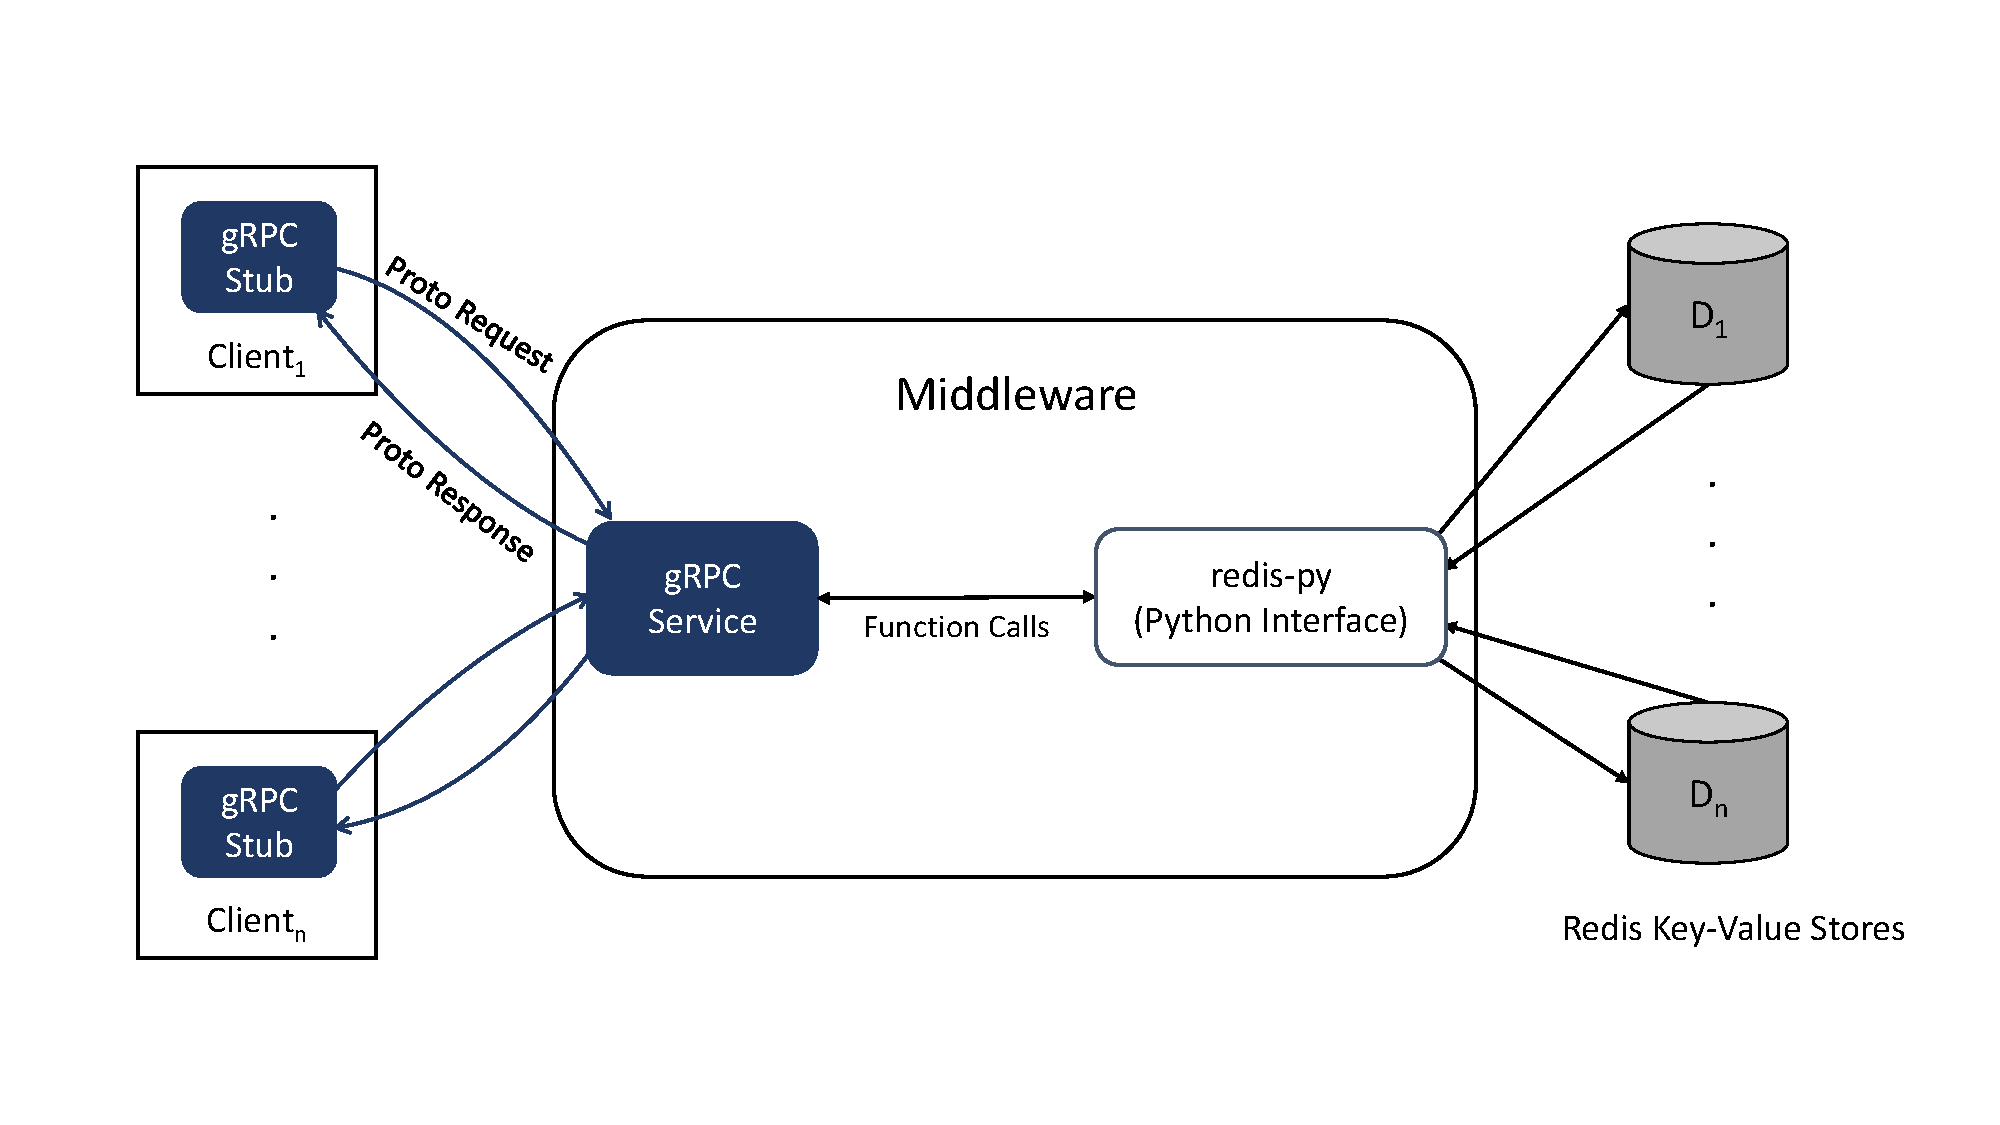
\includegraphics[scale = 0.45]{gfx/design/communication.pdf}}{\caption{Middleware Communication Overview}\label{communication}}
\end{figure}





%***************************************************************************
\section{Design Limitations}
\label{sys_design_limits}

%***************************************************************************
